%\chapter{Muerte y Castigo Póstumo}

\begin{figure}[!hbp]
\centering
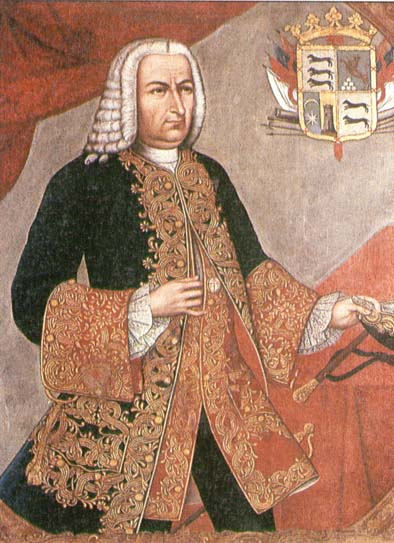
\includegraphics[width=.35\textwidth]{jpg_Sebastian_de_Eslava.jpg}
\caption{\label{fig:eslava} Sebastián de Eslava, virrey de Nueva
  Granada y responsable de la defensa de Cartagena de Indias. Militar
  veterano y ambicioso político, mantuvo un tensa relación con Lezo
  que llevó finalmente a pedir su castigo por sus acciones durante el
  asedio de la ciudad, que obtuvo cuando Lezo ya había fallecido.}
\end{figure}

El 4 de abril, el día que los británicos habían comenzado el bombardeo
sistemático del castillo de San Luis de Bocachica, uno de los que
protegía la ciudad, una bala de cañón había impactado en la mesa del
Galicia en torno a la que estaban reunidos los mandos españoles en
junta de guerra. Las astillas de la mesa hirieron en el muslo y en una
mano a Lezo; la infección de estas heridas le acabó causando la
muerte. La mala relación entre Lezo y el virrey Sebastián de Eslava,
jefe de la plaza y responsable de su defensa, se agudizó una vez
levantado el cerco británico. El primero había abogado constantemente
por adoptar medidas más ofensivas y por acosar al enemigo, mientras
que el segundo había mantenido una actitud más prudente y defensiva,
que para el marino pareció inactividad y desidia en la defensa.

Lezo, cada vez más enfermo, apenas abandonó su residencia a partir del
20 de mayo y mantuvo una guerra epistolar con el virrey, tratando de
defender su actuación durante el asedio, por la que el virrey llegó a
solicitar y obtener el castigo del rey para el marino.116 Lezo intentó
que se reconociese su carrera mediante la obtención de un título
nobiliario, petición para la que recabó el apoyo de José Patiño y de
parte de sus compañeros de armas de la Armada,\index{armada} pero que
el rey, que había recibido los informes desfavorables del virrey y de
otros adversarios de Lezo, rechazó. Blas de Lezo \index{Blas de Lezo}
falleció en Cartagena de Indias \index{Cartagena!de Indias} de «unas
calenturas, que en breves días se le declaró tabardillo» a las ocho de
la mañana del 7 de septiembre. Fue el único de los principales
protagonistas del asedio de Cartagena que no obtuvo recompensa alguna
por sus acciones. Su destitución como jefe del apostadero y la orden
de que regresase a la península ibérica para ser reprendido se aprobó
el 21 de octubre. El rey Carlos III recompensó al hijo de Lezo por las
acciones de su padre, nombrándolo marqués de Ovieco en 1760. Se
desconoce dónde fue enterrado, ya que las fuentes indican distintos
lugares posibles: la iglesia de la Orden Tercera, la capilla de la
Vera Cruz, aneja al convento de San Francisco, o la catedral de
Cartagena.

\section{El Puerto de Santa María y Blas de Lezo}

La estancia de los Lezo en El Puerto de Santa María tuvo varias
fechas. El almirante ya había estado en 1719-20 y en 1730 en Cádiz. De
allí partió, ya viviendo en El Puerto de Santa María, el 3 de febrero
de 1737 hacia Cartagena dirigiendo la que sería la última carrera de
Indias y donde encontraría, como ya se ha reflejado, su fatal destino.

Tras las investigaciones realizadas en los padrones de la época de la
iglesia Mayor Prioral portuense, se ha constatado que Blas de Lezo, su
mujer, sus hijos y un criado afroamericano llamado Antonio Lezo,
vivieron desde 1736 en una casa de la calle Larga, para ser más
exactos en Larga, 70, hoy reconvertida en apartamentos de
alquiler. Tras su muerte, su viuda ---conocida en la localidad como «La
Gobernadora»--- y sus hijos permanecieron en ella hasta la muerte de
ésta el 31 de marzo de 1743.

Josefa Pacheco fue enterrada en el convento de Santo Domingo, sito en
la calle del mismo nombre. A partir de esta fecha, los descendientes
de Blas de Lezo desaparecen de los padrones portuenses.

Durante su residencia en la ciudad, el Cabildo Municipal, siendo
conocedor del prestigio del almirante, hizo a su familia diferentes
concesiones, entre las que destacó una toma de agua para la casa.

Hasta hace pocos años, la ciudadanía portuense siguió llamando a la
mansión casa de «La Gobernadora».